\documentclass[border=5mm]{standalone}
\usepackage[utf8]{inputenc}
\usepackage[T1]{fontenc}
\usepackage{amsmath}
\usepackage{tikz}
\usepackage{pgfplots}
\pgfplotsset{compat=1.18}
\usetikzlibrary{arrows.meta}
\definecolor{utnblue}{RGB}{0, 51, 102}

% Ej8: x(t)=1 en [0,1], h(t)=t en [0,2]
% y(t) = t^2/2  (0<=t<=1),  t-1/2  (1<t<=2),  (3-t)(1+t)/2  (2<t<=3)

\begin{document}
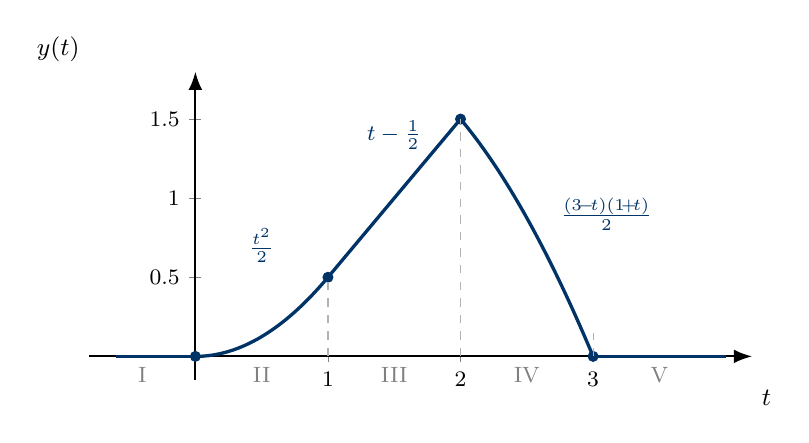
\begin{tikzpicture}[>=Latex, font=\small]

\begin{axis}[
    width=10cm, height=5.5cm,
    axis lines=center,
    xlabel={$t$},
    ylabel={$y(t)$},
    xlabel style={anchor=north west, at={(axis description cs:1,0)}},
    ylabel style={font=\small, rotate=0, anchor=south east, at={(axis description cs:0,1)}},
    xmin=-0.8, xmax=4.2,
    ymin=-0.15, ymax=1.8,
    clip=false,
    axis line style={->, thick},
    xtick={0,1,2,3},
    ytick={0,0.5,1,1.5},
    every tick label/.style={font=\footnotesize},
]
    % Zona I: y=0 for t<0
    \addplot[domain=-0.6:0, samples=2, very thick, utnblue] {0};
    % Zona II: y = t^2/2 for 0<=t<=1
    \addplot[domain=0:1, samples=80, very thick, utnblue] {x^2/2};
    % Zona III: y = t - 1/2 for 1<t<=2
    \addplot[domain=1:2, samples=80, very thick, utnblue] {x - 0.5};
    % Zona IV: y = (3-t)(1+t)/2 for 2<t<=3
    \addplot[domain=2:3, samples=80, very thick, utnblue] {(3-x)*(1+x)/2};
    % Zona V: y=0 for t>3
    \addplot[domain=3:4, samples=2, very thick, utnblue] {0};
    
    % dots at key points
    \fill[utnblue] (axis cs:0, 0) circle (2pt);
    \fill[utnblue] (axis cs:1, 0.5) circle (2pt);
    \fill[utnblue] (axis cs:2, 1.5) circle (2pt);
    \fill[utnblue] (axis cs:3, 0) circle (2pt);
    
    % dashed vertical guides
    \draw[dashed, gray!60, thin] (axis cs:1, 0) -- (axis cs:1, 0.5);
    \draw[dashed, gray!60, thin] (axis cs:2, 0) -- (axis cs:2, 1.5);
    \draw[dashed, gray!60, thin] (axis cs:3, 0) -- (axis cs:3, 0.15);
    
    % zone labels
    \node[font=\footnotesize, gray] at (axis cs:-0.4, -0.12) {I};
    \node[font=\footnotesize, gray] at (axis cs:0.5, -0.12) {II};
    \node[font=\footnotesize, gray] at (axis cs:1.5, -0.12) {III};
    \node[font=\footnotesize, gray] at (axis cs:2.5, -0.12) {IV};
    \node[font=\footnotesize, gray] at (axis cs:3.5, -0.12) {V};
    
    % equation annotations
    \node[font=\footnotesize, utnblue] at (axis cs:0.5, 0.7) {$\frac{t^2}{2}$};
    \node[font=\footnotesize, utnblue] at (axis cs:1.5, 1.4) {$t-\frac{1}{2}$};
    \node[font=\footnotesize, utnblue, align=center] at (axis cs:3.1, 0.9) {$\frac{(3\!-\!t)(1\!+\!t)}{2}$};
\end{axis}

\end{tikzpicture}
\end{document}
